\documentclass{standalone}
\usepackage{tikz, tikz-cd}
\usetikzlibrary{shapes, decorations.markings}
\begin{document}

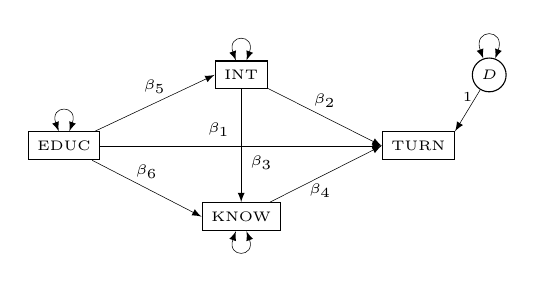
\begin{tikzpicture}[scale=0.9]
\node[draw] (o1) at (6,3) {\tiny{TURN}};
\node[draw] (p2) at (3.5,4) {\tiny{INT}};
\node[draw] (p3) at (3.5,2) {\tiny{KNOW}};
\node[draw] (p1) at (1,3) {\tiny{EDUC}};
\node[draw, circle, inner sep=2] (d1) at (7,4) {\tiny{$D$}};
\draw [->, very thin, >=latex] (p1)--(o1.west) node [midway, above, xshift=-8] {\tiny{$\beta_1$}};
\draw [->, very thin, >=latex] (p2)--(o1.west) node [midway, above] {\tiny{$\beta_2$}};
\draw [->, very thin, >=latex] (p2)--(p3.north) node [midway, right, yshift=-6] {\tiny{$\beta_3$}};
\draw [->, very thin, >=latex] (p3)--(o1.west) node [midway, below, xshift=-2] {\tiny{$\beta_4$}};
\draw [->, very thin, >=latex] (p1)--(p2.west) node [midway, above] {\tiny{$\beta_5$}};
\draw [->, very thin, >=latex] (p1)--(p3.west) node [midway, above] {\tiny{$\beta_6$}};
\draw [->, very thin, >=latex] (d1)--(o1.north east) node [midway, above] {\tiny{1}};
% Residuals:
\draw[<->, very thin, >=latex] (p1) to [out=70,in=110,looseness=7] (p1);
\draw[<->, very thin, >=latex] (p2) to [out=70,in=110,looseness=7] (p2);
\draw[<->, very thin, >=latex] (p3) to [out=250,in=290,looseness=7] (p3);
\draw[<->, very thin, >=latex] (d1) to [out=70,in=110,looseness=7] (d1);
\end{tikzpicture}

\end{document}